\chapter{Examples}\label{chap:examples}

\section{Encryption Process}

In accordance with Kerchoff's principle, the method of encrypting a message was known by the Polish and British cryptologists attempting to break the cipher. In this paper, we will touch on two (2) separate methods of encrypting a message that were used during World War II. The first method was common practice until September 1938, when Germany decided to increase security by changing to the second method, which was used from then on.

\section{Encryption Process Pre-1938}\label{sec:encprocess1938}

Prior to the security changes in 1938, the process for encryption stayed mostly static. The encipherer, person who wanted to encrypt a message, would begin by setting their machine to the daily settings found in the widely dispersed table of keys, say "JEF". These daily settings would correspond to initial settings of the rotors, which would show an alphabetic character on top of the machine, as well as the settings of the plugboard. From there, the encipherer would choose their own individual key, which was supposed to be a random set of three (3) characters that was unique to the individual message, say "KCB". They would type their individual key into the Enigma machine twice, "KCBKCB" thus encrypting it twice using the daily settings, resulting in 6 distinct characters "BQROMP". They typed it twice so as to ensure that there were no errors in encrypting the key, similar to how websites ask for a password confirmation on creation of a password. After encrypting the password using the daily settings, the encipherer would set the machine to their individual key, "KCB" and encrypt the actual message. \cite{wt06}. The six indicator letters would sit as a preamble to the rest of the message.

In order to decipher the message received, the decipherer would follow an almost identical process. They would set their machine to the daily key, and type the first six (6) letters of the message, "BQROMP", into the machine. This would reveal the individual key, "KCB". After ensuring that it was error-free, the decipherer would set their machine to the individual key, and type in the rest of the message to reveal the plain text. Note that the same machine, with the same internal hardware, is used to both encrypt and decrypt the message.

\section{Mathematical Theory Behind Cracking Enigma}\label{sec:maththeory}

The initial goal in cracking the Enigma machine was to determine the hardware connections on the rotor closest to the keyboard. Knowing the hardware connections on that rotor would allow the Polish mathematicians to reconstruct their own Enigma machine, and use that to decrypt more messages. It would open the doors for more rapid and widespread decryption.

Of course, it was not easy to find out what the hardware connections on the rotor were. All the mathematicians had to work with were ciphertexts that had been intercepted throughout the day, so they could only attempt ciphertext-only attacks. However, Polish mathematicians Marian Rejewski, Jerzy Rozycki, and Henryk Zygalski were able to crack the Enigma cipher in 1932. The solution to this believed 'impossible' problem took its roots in the permutation theory that was covered in \secref{sec:mathconcepts}, with some help from the enciphering process itself, covered in \secref{sec:encprocess1938}.

Since every message was encrypted with a different individual key, coupled with the fact that each rotor rotated at different speeds, it was impossible to determine the plain text just by comparing ciphertexts. However, with knowledge of the encryption process, it was possible to draw conclusions about the first six (6) letters of each ciphertext, and with enough ciphertexts, draw conclusions about the inner workings of the Enigma machine. The mathematicians knew that the first six (6) letters were a repeat of the same three (3) letter key, they could draw two conclusions.

\begin{enumerate}
\item All message keys started from the same position, determined from a common set of keys.
\item The first letter in the plaintext was the same as the fourth, the second the same as the fifth, and the third the same as the sixth.
\end{enumerate}

This is where permutation theory comes in. In this section of the paper, we will make reference to permutations $A$ - $F$, which correspond in kind to a different substitution cipher created by Enigma. $A$ corresponds to the transposition of letters (of the form $(ab)(cd)(ef)...$ where each letter occurs once) that occurs on the very first keypress in an encryption, which correlates to the first value in the encipherer's individual key. $B$ then corresponds to the transposition that occurs on the second keypress, $C$ on the third, and so on. One will notice that $A$ and $D$ both correspond to the first value in the encipherer's individual key, $B$ and $E$ correspond to the second, and $C$ and $F$ correspond to the third. This was one of the first conclusions drawn by the Polish mathematicians as well.

The first step to cracking Enigma involved gathering as many ciphertexts as possible and recognizing products of permutations within them. We know that $A$ and $D$ correspond to the same letter. This means that when the encipherer types a character $x$, he obtains the value $a$ as his ciphertext, and when he types the same character $x$ for the double enciphering of his individual key (in the fourth place), he obtains the value $b$, indicating a relationship between the values $a$ and $b$. This relationship between keys here can be modeled as a product of permutations $AD$, which is the product of the individual permutations $A$ and $D$.

As an example, take the ciphertexts

\begin{CVerbatim}[fontsize=\small]
dmq vbn
von puy
puc fmq
\end{CVerbatim}

One can see that $d \rightarrow v$, $v \rightarrow p$, and $p \rightarrow f$. That means that the permutation $AD$ contains $dvpf$. The same process can be applied to see that $oumb$ is in $BE$ and $cqny$ is in $CF$. If enough ciphertexts are gathered such that each letter of the alphabet is seen in each position at least once, entire permutations can be constructed. The permutation sets created from the daily ciphertexts are called the 'characteristic' for the day \cite{wk85}.

\begin{figure}[h!]
\begin{centering}
  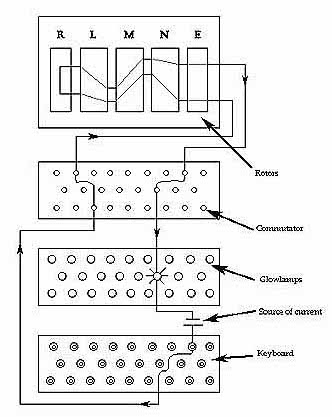
\includegraphics[height=6.5cm]{images/permutations.jpg}
  \caption{Electric Current Through Enigma}
  \label{fig:current1}
\end{centering}
\end{figure}

Next, it is important to understand how the machine works, with regards to a circuit. \figref{fig:current1} shows the circuit that is created when a key is pressed. If we label the commutator (or plugboard) as $S$, the three rotors from left to right as $L$, $M$, $N$ respectively, and the reversing drum $R$, we can represent the path of the current as the product of the permutations $SNMLRL^{-1}M^{-1}N^{-1}S^{-1}$. However, we also need to account for the fact that the $N$ rotor revolving $1/26th$ of a turn each time a key is pressed, and we can represent that with the permutation $P = (abcdefghijklmnopqrstuvwxyz)$. Thus, if the $N$ rotor rotates twice, we will have $P^2$, and so on and so forth. With this, we can rewrite the previous equation for each individual keypress, including $P$.

$$A = SPNP^{-1}MLRL^{-1}M^{-1}PN^{-1}P^{-1}S^{-1}$$
$$B = SP^2NP^{-2}MLRL^{-1}M^{-1}P^2N^{-1}P^{-2}S^{-1}$$
$$C = SP^3NP^{-3}MLRL^{-1}M^{-1}P^3N^{-1}P^{-3}S^{-1}$$
$$D = SP^4NP^{-4}MLRL^{-1}M^{-1}P^4N^{-1}P^{-4}S^{-1}$$
$$E = SP^5NP^{-5}MLRL^{-1}M^{-1}P^5N^{-1}P^{-5}S^{-1}$$
$$F = SP^6NP^{-6}MLRL^{-1}M^{-1}P^6N^{-1}P^{-6}S^{-1}$$

It is clear that $MLRL^{-1}M^{-1}$ is repeated in every one of these equations, so we can replace that value with the value $Q$. \cite{wk85} We also must calculate the products $AD$, $BE$, and $CF$ with respect to the above equations, and we get the following equations:

$$AD = SPNP^{-1}QPN^{-1}P^3NP^{-4}QP^4N^{-1}P^{-4}S^{-1}$$
$$BE = SP^2NP^{-2}QP^2N^{-1}P^3NP^{-5}QP^5N^{-1}P^{-5}S^{-1}$$
$$CF = SP^3NP^{-3}QP^3N^{-1}P^3NP^{-6}QP^6N^{-1}P^{-6}S^{-1}$$

In order to solve these equations, we can take one of two routes. One, we can solve for $S$, $N$, and $Q$ using $AD$, $BE$, and $CF$. Two, we can solve for $A$ - $F$, $S$, $Q$, and $N$. One may notice that there are more unknowns than equations, which makes these sets impossible to solve. This is where the Polish mathematicians hit a stopping point. That is, until Capt. Gustave Bertrand was able to provide the Polish Cipher Bureau with some key tables that had recovered from the Germans \cite{wk85}. This gave the Polish mathematicians the values of $S$ that they needed. They were also able to determine $A$ - $F$ based on encipherer's habits, and applications of the converse Theorem on the Product of Transpositions discussed in \secref{sec:mathconcepts}. Therefore, the four (4) unknowns from the equations was reduced to two (2), which is solvable.

$$SAS^{-1} = PNP^{-1}QPN^{-1}P^{-1}$$
$$SBS^{-1} = P^2NP^{-2}QP^2N^{-1}P^{-2}$$
$$SCS^{-1} = P^3NP^{-3}QP^3N^{-1}P^{-3}$$
$$SDS^{-1} = P^4NP^{-4}QP^4N^{-1}P^{-4}$$
$$SES^{-1} = P^5NP^{-5}QP^5N^{-1}P^{-5}$$
$$SFS^{-1} = P^6NP^{-6}QP^6N^{-1}P^{-6}$$

$N$ and $Q$ were able to be solved using the known values, and the resulting $N$ permutation corresponded to the connectors in that specific rotor \cite{wk85}. That $N$ was the result the mathematicians were after, and it was this permutation that was integral to continuous decryption of messages throughout the 1930s.

\section{Encryption Process Post-1938}

Germany realized that their messages were being successfully intercepted and decrypted. To throw off their enemies, they added some complexities to the Enigma machines and the practices of using it. First, they added two rotors to the existing three. This increased the combination of rotor positions from six (6) to sixty (60). Previously, the Poles had six (6) Bomby, one for each possible combination of rotor positions, that would iterate over rotation settings for the given position in an effort to find the keys to messages of the day. The increase in hardware complexity rendered this method essentially obsolete. The Germans also recognized the fault in double-enciphering message keys, so they replaced that practice as well. Rather than starting with a network-wide common setting, clerks would choose three random letters, say "WER", and use this as their initial setting. Choosing three more random letters still, "IUY", the clerk would encrypt this indicator only once, giving "BSD". The new preambles would be comprised of the initial setting, followed by the encrypted indicator, "WERBSD". This troubled the Ultra team at Bletchley Park for a time, until they began to find patterns and habits in the clerks' use of the machines. They were lazy and would use letter combinations that did not require much thought: repeating letters, ones that sat next to each other on the keyboard, or names. Sometimes the clerks would not change the settings between messages at all and would simply use the ending state of their machine from one message as the beginning stage for a new one \cite{mf01}. These habits, dubbed "cillies" by Bletchley Park, are what allowed the team to reframe their approach to deciphering messgaes.

\section{Cryptological Machines}

It was not enough to find the mathematic solutions to Enigma messages. The complexity of the machine and its many possible settings required too much time to complete by hand and effectively intercept and interpret messages into actionable strategies for those resisting and eventually fighting Nazi Germany. The cyclometer, previously mentioned, was one of the very first mechanical aides that helped cut down on the time required for deciphering. Other, still manual, tools such as perforated sheets depicted relationships between the double encrypted keyspaces helping to find the encoded key. By far the greatest accomplishment in accelerating this process was the development of the Crytological Bomb. In Polish shortened to Bomba, the machine would iterate over the possible rotations of Enigma's rotors, given the rotor order. Up until 1938, this was a monumental improvement and enabled the team to successfully decipher 75\% of messages intercepted, including those messages which came riddled with errors. After Germany increased the number of rotors, and increased the total of all rotor combinations tenfold, the Bomba became unusable. This was also around the time which knowledge and information was transferred from the Polish to the French and British. Quickly, the British began developing their own Cryptological Bomb, Bombe for short. The electromechanical system ran quite similar to the Bomba, but instead of only being able to operate as if it were a single Enigma machine, it could run as if 36 were joined together. Additionally, the overall algorithm is what made it stand apart and gave the edge back to the enemies of Nazi Germany. Rather than focus on the encoded key itself, the Bombe evaluated the entire ciphertext, searching for a "crib", a commonly used word that could be reasonably be expected to occur in the message. Given a crib, the cryptanalysts would map out a possible connection of the crib to ciphertext, and then they would run the Bombe to verify their mapping and find the related key that would render the cipher text from the crib. Once the key was obtained, they could decipher the remaining message.
